% \iffalse
\let\negmedspace\undefined
\let\negthickspace\undefined
\documentclass[journal,12pt,twocolumn]{IEEEtran}
\usepackage{cite}
\usepackage{amsmath,amssymb,amsfonts,amsthm}
\usepackage{algorithmic}
\usepackage{graphicx}
\usepackage{textcomp}
\usepackage{xcolor}
\usepackage{txfonts}
\usepackage{listings}
\usepackage{enumitem}
\usepackage{mathtools}
\usepackage{gensymb}
\usepackage{comment}
\usepackage[breaklinks=true]{hyperref}
\usepackage{tkz-euclide}
\usepackage{listings}
\usepackage{gvv}
\def\inputGnumericTable{}
\usepackage[latin1]{inputenc}
\usepackage{color}
\usepackage{array}
\usepackage{longtable}
\usepackage{calc}
\usepackage{multirow}
\usepackage{hhline}
\usepackage{ifthen}
\usepackage{lscape}

\newtheorem{theorem}{Theorem}[section]
\newtheorem{problem}{Problem}
\newtheorem{proposition}{Proposition}[section]
\newtheorem{lemma}{Lemma}[section]
\newtheorem{corollary}[theorem]{Corollary}
\newtheorem{example}{Example}[section]
\newtheorem{definition}[problem]{Definition}
\newcommand{\BEQA}{\begin{eqnarray}}
\newcommand{\EEQA}{\end{eqnarray}}
\newcommand{\define}{\stackrel{\triangle}{=}}
\theoremstyle{remark}
\newtheorem{rem}{Remark}
\begin{document}

\bibliographystyle{IEEEtran}
\vspace{3cm}

\title{NCERT Discrete Assignment}
\author{EE23BTECH11007 - Aneesh Kadiyala$^{*}$% <-this % stops a space
}
\maketitle
\newpage
\bigskip

\renewcommand{\thefigure}{\theenumi}
\renewcommand{\thetable}{\theenumi}
%fi

\vspace{3cm}
\textbf{Question 10.5.2.19:} Subba Rao started work in 1995 at an annual salary of Rs. 5000 and received an increment of Rs. 200 each year. In which year did his income reach Rs. 7000?
\\
\solution
\begin{enumerate}
\item
Let Subba Rao's initial salary $a_0$ = Rs. 5000
\\
Let Subba Rao's increment $d$ = Rs. 200
\\
Subba Rao's salary after n years = $a_n$ = $a_0 + (n - 1)d$
\\
\[7000 = 5000 + (n - 1)(200)\]
\[2000 = (n - 1)(200)\]
\[n = 11\]

$\implies$Subba Rao's income reaches Rs. 7000 eleven years after he started working.

Therefore, Subba Rao's income reached Rs. 7000 in the year 2006.

\item \textbf{Finding $x(n)$}

The series is an arithmetic progression.
\[x(n) = x(1) + (n - 1)d\]
where $d$ is the common difference.

It is given that initial value $x(1)$ is 5000 and common difference $d$ is 200.
\[\implies x(n) = 5000 + (n - 1)(200)\]
\[\implies x(n) = 4800 + 200n\]

\begin{figure}[h!]
    \centering
    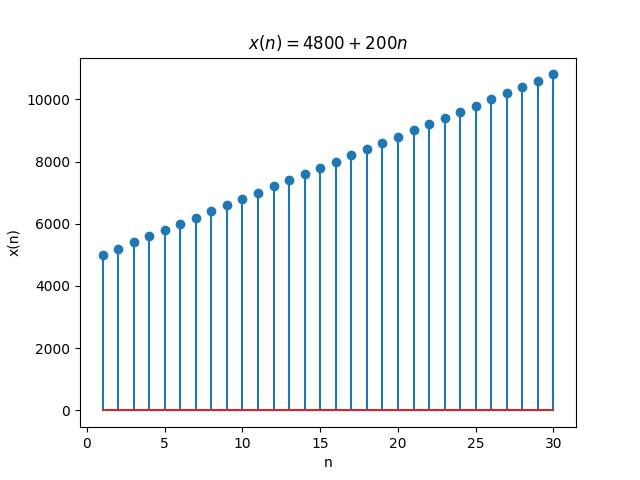
\includegraphics[width=\columnwidth]{plots/10_5_2_19.png}
\end{figure}

\item \textbf{Z-transform of $x(n)$}

Let Z-transform of $x(n)$ be $X(z)$.

\[X(z) = \sum_{n = -\infty}^{\infty} x(n)z^{-n}\]
\[X(z) = \sum_{n = 1}^{\infty} (4800 + 200n)z^{-n}\]
\[X(z) = 4800\lim_{n\to\infty}\sum_{i = 1}^{n}z^{-i} + 200\lim_{n\to\infty}\sum_{i = 1}^{n}iz^{-i}\]

\begin{enumerate}
\item If $|z| > 1$:
\[X(z) = \frac{4800z^{-1}}{1 - z^{-1}} + 200(\frac{z^{-1}}{1 - z^{-1}} + \frac{z^{-1}}{(1-z^{-1})^2})\]
\[X(z) = \frac{4800}{z-1} + 200(\frac{1}{z-1} + \frac{z}{(z - 1)^2})\]
\[{X(z) = 5000(z - 1)^{-1} + 200z(z-1)^2}\]

\item If $|z| \le 1$:
\[X(z) \to \infty\]

\end{enumerate}

Region of Convergence (ROC) of $z$ is $|z| > 1$.

\end{enumerate}

\vspace{1cm}
\textbf{Question 11.9.3.30:} The number of bacteria in a certain culture doubles every hour. If there were 30 bacteria present in the culture originally, how many bacteria will be present at the end of $2^{nd}$ hour $4^{th}$ hour and $n^{th}$ hour?
\\
\solution
\begin{enumerate}
\item
Let number of bacteria initially be $a_0$ = 30
\\
Let number of bacteria at the end of $n^{th}$ hour be $a_n$.
\\
Since number of bacteria doubles every hour, \[a_n = 2a_{n - 1}\]
\[a_n = 2(2a_{n - 2})\]
\[\dots\]
\[a_n = 2^na_0 = 2^n(30)\]
$\implies a_2 = 2^2(30) = 120$ and $a_4 = 2^4(30) = 480$
\\

Therefore, number of bacteria at the end of the $2^{nd}$ hour is 120, $4^{th}$ hour is 480, and $n^{th}$ hour is $30(2^n)$.

\item \textbf{Finding $x(n)$}

The series is a geometric progression.
\[x(n) = x(1) (r^{n-1})\]
where $r$ is the common ratio.\\
From the solution, $x(1) = 30$, $r = 2$.
\[\implies x(n) = 30(2^{n-1})\]
\[\implies x(n) = 15(2^n)\]

\begin{figure}[h!]
    \centering
    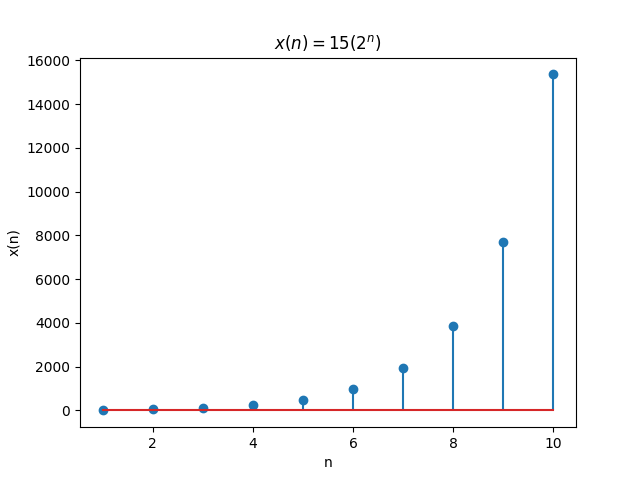
\includegraphics[width=\columnwidth]{plots/11_9_3_30.png}
\end{figure}


\item \textbf{Z-transform of $x(n)$}

Let Z-transform of $x(n)$ be $X(z)$.
\[X(z) = \sum_{n = -\infty}^{\infty} x(n)z^{-n}\]
\[X(z) = \sum_{n = 1}^{\infty} (15)(2^n)(z^{-n})\]
\[X(z) = 15\lim_{n\to\infty}\sum_{i = 1}^{n}(\frac{2}{z})^i\]

\begin{enumerate}
\item If $|z| > 2$:
\[X(z) = 15\frac{\frac{2}{z}}{1 - \frac{2}{z}}\]
\[X(z) = 30(z - 2)^{-1}\]

\item If $|z| \le 2$:
\[X(z) \to \infty\]

\end{enumerate}

Region of Convergence (ROC) of $z$ is $|z| > 2$.

\end{enumerate}
\end{document}